\chapter{Functional Paradigms}
\section{Functional Programming}
Mutation is where an attribute of a variable can change while the identity of the variable is maintained.  For example, could define a polynomial class, then set a certain coefficient to a particular value.

Functional programming is a programming strategy that avoids mutation/reliance on state information. Immutable values are used. These can be transformed, but the idea is to minimise side effects. We don't want to pass an argument to a function that will then modify that argument. Input goes in, return value comes out with inputs unchanged.

The restricted definition of a functional programming framework is one in which there are no mutable variables, assignments, or imperative conttrol structures
In a wider sense, functional programming can be carried out in any language that allows the construction of elegant programs that focus on functions

In scala, functions are first class objects. They can be treated and passed around just like any other variable (as in python)


\section{call-by-name, call-by-value}
Functions arguments in scala can be handled two ways. The argument can be called by name, or called by value.

\begin{lstlisting}
//call by value
def CBVfunc(a:Int):Int = {...}
\end{lstlisting}
Function CBVfunc takes an int, returns an Int. The integer argument a is evaluated when the function is called.


\begin{lstlisting}
//call by name
def CBNfunc(a: =>Int): Int = {...}
\end{lstlisting}
Function CBNfunc takes an integer argment (a), which is evaluated when it needs to be (or not at all!).

Not all functions terminate, infinte loops are a thing

Both call by value and call by name will reduce to the same outcome provided
\begin{itemize}
  \item the reduced expression consists of pure functions (no state information/side effects?)
  \item both evaluations terminate (no infinte loops)
\end{itemize}

if call by value terminates, then call by name will also
converse is not guarenteed: call by name termination does not imply call by value termination
in call by name, unused arguments are not evaluated
\begin{itemize}
  \item could have a function that takes two arguments. The second argument is not used (always)
  \item could pass a non-terminating input to the CBN function, which is not used. no big deal
  \item call by value will try to evaluate it and get stuck
\end{itemize}

Below is an example of a function that will terminate when arguments are called by name but not when called by value.
\begin{lstlisting}
// an infinite loop, this run indefinitely when evaluated
def loop = loop 

// call by value function, arguments are evaluated once when the function is called
def mooseCBV(a: Int, b: Int):Int = a

// this evaluates loop, starting the infinte loop...
mooseCBV(1,loop)

// same as above, but using call-by-name (=>)
def mooseCBN(a: =>Int, b: => Int) = a

// returns 1, the loop is not evaluated
mooseCBN(1,loop)
\end{lstlisting}

Scala uses call by value by default, unless the function arguments are defined with \verb|=>|


\section{Conditionals}
Boolean operations don't always need to evaluate the right hand operand (short circuit evaluation)

\begin{verbatim}
true && e -> e
false && e -> false
true || e -> true
false || e -> e
\end{verbatim}

Things can be defined by name or by value.
so \lstinline|def x = loop| is a function, it is not evaluated untill it needs to be (call by name). 

\lstinline|val x = loop| evaluates to loop (call by value) immediately. this will kill your scala session/repl.

\section{Recursion}
Recursive functions must always have their return type explicitly defined (to make the compiler's life easier).

\subsection{Tail Recursion}
If a function calls itself as its last action, the stack frame can be reused
Essentially it acts the same as a loop

If a functions last action is to call a function, (maybe the same, maybe different function), then the stack frame can be used - this is a tail-call (tail recursion is recursive tail-calling).

Tail recursive factorial example(works)

\begin{lstlisting}
def factorial(N:Int) = {
    @scala.annotation.tailrec
    def currentProd(n:Int, prod:Int) :Int = {
        if (n==0) prod
        else currentProd(n-1,n*prod)
    }
    currentProd(N,1)
}
\end{lstlisting}

A lot of loops can be replaced by tail recursion. Usually this involves defining an inner function for the actual recursion, which accepts an accumulator argument in addition to other parameters. Recursive invocations of the inner function pass the current value of the accumulator, or return something when termination condition is met. For tail recursion (or recursion in general), it seems helpful to define the termination conditions at the very begining, then figure out the remaining logic.

\section{Blocks and Scope}
A block is defined by curly braces \lstinline|{}|

Definitiones inside a block are invisible outside the block. 
Definitions from outside the block are visible inside, provided they have not been shadowed.
A lot of object oriented functionality can be warngled from scopes and closures. Methods defined within a class constructor have acesss to the parameters of that constructor, even if those parameters are not assigned to fields of the class. 
For example:

\begin{lstlisting}
class NonEmpty(elem: Int, left: IntSet, right: IntSet) extends IntSet {
  def contains(x: Int): Boolean = if (x < elem) left.contains(x)
    else if (x > elem) right.contains(x)
    else true
    ...
\end{lstlisting}
the method \lstinline{contains} refers to \lstinline{elem}.

\section{higher order functions}
% TODO - clean below here
functions are first class values
they can be passed and returned
a function that does this is called a higher order function

this can be used to factor out common procedures. For example, 
\begin{lstlisting}
sumFunc(a:Int,b:Int,f: Int =>Int): Int = {
    if (a > b) 0 else f(a) + sumFunc(a+1,b,f)
}
\end{lstlisting}

defines a function sumFunc, that takes two integers and a function that takes an Int and returns an Int (\lstinline{Int => Int})
For example, we could sum all squares or cubes between 2 and 5 by calling
\begin{lstlisting}
sumFunc(2,5,square)
sumFunc(2.5.cube)
\end{lstlisting}
The notation \lstinline{A => B} is  a {\b function type}. it is a type that defines a mapping from type {\b A} to type {\b B} (by a function)

\section{anonymous functions}
strings exist as literals. We can just write "abc", and the compiler knows it to be a string. We don't need to do \lstinline{def str = "abc"; println(str)}
instead \lstinline|println("abc")| works just fine
Same can be done with functions, we don't always need to define a function, we can define anonymous functions as needed. (same as lambda functions in python)

these are defined like this
\begin{lstlisting}
(x: Int) => x*x*x
\end{lstlisting}
the type of x can be omitted if it can be inferred.

anonymous functions are syntactic sugar:
\lstinline{(x:Int) = x*x} and \lstinline{def f(x:Int) = x*x; f} 
evaluate to the same.

tail recursive sum
\begin{lstlisting}
def sum(f: Int => Int, a:Int, b:Int) = {
    @scala.annotation.tailrec
    def doSum(total:Int, aval:Int):Int = {
        if (aval > b) total else doSum(total + f(aval),aval+1)
    }
    doSum(0,a)
}
\end{lstlisting}

\chapter{currying}
from the scala docs 
\begin{displayquote}
"Methods may define multiple parameter lists. When a method is called with a fewer number of parameter lists, then this will yield a function taking the missing parameter lists as its arguments."
\end{displayquote}

For example, consider a function \verb|sum|, which takes a function \verb|f| and returns a function taking two integers as parameters (the bounds). 
\begin{lstlisting}
def sum (f: Int => Int) :(Int, Int) => Int = {
    def sumF(a:Int,b:Int): Int = {
    if (a>b) 0 else f(a) + sumF(a+1,b)
    }
    sumF
}
\end{lstlisting}

The function sum now takes a function, and returns a function (return type is \lstinline{(Int,Int) => Int}). the returned function will take two Ints and return one. In this case, when an initial function (f) is passed into sum, it will return a function that sums the initial function (f) within the supplied bounds.

so, we could do
\begin{lstlisting}
def sumCubes = sum((x:Int) => x*x*x)
def sumSquares = sum((x:Int) => x*x)
// and then invoke them
sumSquares(2,3) // 13
sumCubes(4,7) // 748
\end{lstlisting}

Alternatively, we could invoke the returned function directly
\begin{lstlisting}
val moose = sum((x:Int)=>x*x) (2,3) //13
\end{lstlisting}

Again, there is some syntactic sugar for currying. For example
\begin{lstlisting}
def sum(f:Int => Int) (a:Int,b:Int): Int = {
    if (a>b) 0 else f(a) + sum(f)(a+1,b)
}
\end{lstlisting}

is equivalent to the definition of sum above, but without the definition of the inner function. When invoked as \lstinline|sum(func)| the return type will be a function that takes two integers as parameters: the bounds a and b of the original sum function (the second parameter list). As mentioned above, when a function taking multiple parameter lists is invoked with one or more parameter lists absent, then the return type is a function that takes the missing parameter lists.

\section{multiple parameter lists}
Functions can be specified with multiple sets of parameter lists

\begin{lstlisting}
def f(args_1)...(args_n) = E
\end{lstlisting}
For $n > 1$, this is equivalent to

\begin{lstlisting}
def f(args_1)...(args_n-1) = {def g(argsn) = E ; g}
// or
def f(args_1)...(args_n-1) = (args_n => E)
\end{lstlisting}

Carrying this through gives
\begin{lstlisting}
def f = (args1 => (args2 => ...(argsn => E)))
\end{lstlisting}
named after Haskell Brooks Curry (same guy Haskell language is named after).

As an example, we can write a function that calculates the product of values of a function for points on an interval.
We can then define a factorial function in terms of these products.

Our original product and factorial functions look like this
\begin{lstlisting}
def product(f: Int=>Int) (a:Int,b:Int) :Int = {
if (a>b) 1 else product(f)(a+1,b)*f(a)  
}

def factorial(n:int) = product((x:Int) =>x)(1,n)
\end{lstlisting}

Now we will use currying to generalise. In this case we will calculate the sum and product of squares (rather than factorials)
\begin{lstlisting}

def CumulativeFunctionOperation(operation: (Int,Int) => Int, initVal:Int)(f:Int=>Int)(a:Int,b:Int):Int = {
    if (a>b) initVal else operation(f(a),CumulativeFunctionOperation(operation,initVal)(f)(a+1,b))
}

def sum2:(Int=>Int)=>(Int,Int)=>Int = CumulativeFunctionOperation((x:Int,y:Int)=> x+y,0)

sum2(x=>x*x)(2,3) // 13

def prod2:(Int=>Int)=>(Int,Int)=>Int = CumulativeFunctionOperation((x:Int,y:Int)=> x*y,1)

prod2(x=>x*x)(2,3) // 36
// factorial
def fact(n:Int) = prod2(x=>x)(1,n)

\end{lstlisting}

CumulativeFunctionOperation is a form of map-reduce. The operation being apply is a reducer (it takes two inputs and returns a single value). The supplied function is the mapper, for sum2 and prod2 this is the anonymous function \lstinline|x=>x*x| which computes squares, for fact this is the identity function \lstinline|x=>x|. The bounds of CFO define the sequence that we are map/reducing. This is pretty neat. These functions are in the worksheet ``curying.sc`` under week2/misc\_worksheets project


\section{Aside - functional implementation of sets}
The week 2 assignment was interesting. A set can be implemented as a function that returns true if it contains the supplied argument. The union of two sets is then the ``or'' of their charateristic functions, and the intersection the ``and''. 
The implementation of a ``map'' function took me a while to figure out. Instead of thinking of map as \lstinline[language=Python]|[f(x) for x in set]|, we define the mapped characteristic as a check to see whether the initial set contains (any) element that would map to x. It's a bit backwards. 
\begin{lstlisting}
def map(s: Set, f: Int => Int): Set = (x:Int) => exists(s,(y:Int)=> f(y) == x)
// exists returns true if any element in the set s satisfies the supplied condition, false otherwise.
\end{lstlisting}
The code for this assignment is under \verb|week2/funsets/src/main/scala/funsets/FunSets.scala|

\chapter{Classes}

Classes are a type of object that contain methods (member functions) and fields (member data). A class representing a rational number is defined below. Some more examples related to classes are in the rational worksheet (\verb|week2/misc\_worksheets/rationals.sc|).

\begin{lstlisting}
class Rational(x:Int, y:Int) {
  def method(args:Int) = block
}
\end{lstlisting}

The class definition is the constructor - a new instance of Rational can be created using \lstinline|val rat = new Rational(2,3)|. Class methods are public by default, private methods should be prefaced with the \lstinline|private| declaration. Overriding methods should be prefaces with the  \lstinline|override| declaration.

In a class method, the instance of the class can be referenced with \lstinline|this| (In lectures, the argument to class methods is often "that", so multiplication could be written \lstinline|new Rational(this.numer*that.numer,this.denom*that.denom)|)

Class fields can be explicitly assigned in the constructor
\begin{lstlisting}
class foo(A: Int) {
  val memberInt = A
}
\end{lstlisting}
or alternatively the fields can be defined implicitly in the constructor - \lstinline|class foo(val memberInt: Int) {}| . Both of these definitions are equivalent.

Instances of a class are objects. This can be ambiguous, as objects are a thing in Scala (see below)

\section{ Aside - require and assert}
Require is a function that can be used to make sure the class being initialised meets some conditions, for example see the rational worksheet (week2/misc\_worksheets/rationals.sc). We {\i require} that a class be initialised with a nonzero denominator. require takes a condition and a string as arguments. If the condition is not met, then an \lstinline|illegalArgumentException| is thrown and the string is printed.

The \lstinline|assert| function behaves similarly. Assert also takes a condition and a string, but throws an AssertionError when the condition is not met. The intent is that require enforces a precondition on the caller of a function, while assert is used to check the code of the function itself. Require is to make sure the function is called as intended, assert is to check that things are not borked in the internals.

\section{Alternate constructors}
Alternate constructors can be created by defining "this" as a function that takes alternate arguments (by signature), and then invoking the primary constructor appropriately (again, using this)
For example, an alternate constructor for Rational could be defined (within Rational) as \lstinline|def this(x:Int) = this(x,1)|. Then \lstinline|val moose = new Rational(3)| will be mapped to \lstinline|Rational(3,1)|.

\section{Objects}

Objects are defined similarly to classes, but using the keyword \lstinline{object} instead of \lstinline{class}. Objects can also inherit from (extend) other classes and traits. The difference is that objects are singleton, that is, only a single instance of an object may be created. Objects may be referenced in the scope they are defined in, or imported from another package.

\subsection{companion objects}
If an object has the same name as a class then it is a companion object. In scala, class or static methods do not exist. Things like class methods can be defined in a companion object, class instances can always access the methods of their companion objects

This example is taken from the scala docs \url{https://docs.scala-lang.org/tour/singleton-objects.html} 
\begin{lstlisting}
import scala.math._
case class Circle(radius: Double) {
  import Circle._
  def area: Double = calculateArea(radius)
}
object Circle {
  private def calculateArea(radius: Double): Double = Pi * pow(radius, 2.0)
}
val circle1 = new Circle(5.0)
circle1.area
}
\end{lstlisting}

Objects can be useful for defining factory methods.

\section{Defining operators/ infix notation}

Any method with a parameter can be used like an infix operator. \lstinline|r add s| is equivalent to \lstinline|r.add(s)|, \lstinline|r less s| to \lstinline|r.less(s)|, etc.

Operators may also be used as identifiers. Valid identifiers in scala can have the following forms
\begin{itemize}
  \item { \b alphanumeric } - starts with letter, followed by letters/numbers
  \item { \b symbolic } - start with operator symbol \lstinline|+:?~#|, followed by other operator symbols
  \item {\b underscore } - counts as letter
  \item {\b alphanumeric } can end in \_ followed by operator symbols
\end{itemize}

so \lstinline|x_, x_+*, x1, *, vector_++, counter_=| are all valid identifiers. Things like \lstinline|+, -, <, >| can just be defined as class methods.

unary operators should be defined using the prefix \lstinline|unary_|. For example, there is a distinction between the binary version of ``-'' (subtraction) and the unary ``-'' (negation). \lstinline|-Foo| is equivalent to \lstinline{Foo.unary_-()}
% unary_- the binary - operator

\section{operator precedence}

Details on operator precedence can be found here: \url{https://docs.scala-lang.org/tour/operators.html}

\begin{lstlisting}
a + b ^? c ?^ d less a ==> b | c
\end{lstlisting}
can be rewritten (parenthesised) as 
\begin{lstlisting}
((a + b) ^? (c ?^ d)) less ((a ==> b) | c)
\end{lstlisting}

\section{Classes, hierarchies, and dynamic binding}
Classes (and objects) can inherit from existing classes or traits. 

\begin{lstlisting}
class baseAdder() {
  def addTwo(x:Int) = x +2
}
class badAdder() extends baseAdder {
  def addThree(x:Int) = x + 4
  override def addTwo(x: Int) = x +1
}
val moose = new baseAdder()
moose.addTwo(2) // Int = 5
val caribou = new badAdder()
caribou.addTwo(1) // Int = 2
caribou.addThree(4) //Int = 8
\end{lstlisting}

\subsection{abstract classes}
Abstract classes, like in c++, are classes with definitions that lack implementations. They are prefaced with the keyword \lstinline|abstract|. If a class is defined as abstract, then it can not be instantiated using \lstinline|new| (compiler will give an error).
\begin{lstlisting}
abstract class IntSet {
    def incl(x:Int): IntSet
    def contains(x:Int) Boolean
    def union(other: IntSet): IntSet
}
\end{lstlisting}

\subsection{traits}
Traits are like interfaces in Java. They can declare methods and fields but provide no implementation. Traits take no parameters, and can not be instatiated. 
\begin{lstlisting}
trait Pet {
  val name: String
}
\end{lstlisting}

\subsection{subtyping}
We use the extend keyword to derive a class.
\begin{lstlisting}
class NonEmpty(elem: Int, left: IntSet, right: IntSet) extends IntSet {
  def contains(x: Int): Boolean = if (x < elem) left.contains(x)
    else if (x > elem) right.contains(x)
    else true
  def incl(x:Int): IntSet = if (x < elem) new NonEmpty(elem,left.incl(x), right)
    else if (x > elem)  new NonEmpty(elem,left, right.incl(x))
    else this
  override def toString = s"{ ${left} ${elem} ${right} }"
  override def union(other: IntSet) = left.union(right).union(other).incl(elem)
}
class Empty extends IntSet {
  def contains( elem: Int): Boolean = false
  def incl(x:Int): IntSet = new NonEmpty(x,new Empty, new Empty)
  override def toString = "."
}
\end{lstlisting}
this implies that both empty and nonempty meet all the criteria of intset (implement union, contains and incl), but may have additional functionality. Instances of thee classes can be used whenever IntSets are required. IntSet is the {\bf superclass} of both Empty and NonEmpty (which are {\bf subtypes} of IntSet). If no extend clause is given when defining a class, then the standard java class "object" is assumed. 

In java and scala a class can only have one superclass (not true in python or c++). A class may only extend from a single class (or trait). If there are several natural (potential) superclasses, use traits instead.
\begin{lstlisting}
trait Planar {
  def height: Int
  def width: Int
  def surface = width*height
}
class Square extends Shape with Planar with Movable with ...
\end{lstlisting}

% the base class of a given class are all direct or indirect superclasses

% redefine can be used to reimplement a non abstract definition, but the override clause must be used.
\subsection{dynamic binding}
Scala can use dynamic binding. The type of an object is determined at runtime. For example, a function $f$ may take an instance of class A as an argument, and invoke \lstinline|A.method()|. There may be a subclass B derived from A, which can override \lstinline{A.method()}. At runtime, the type of the object passed to $f$ is checked, and either A.method or B.method is invoked. Static binding is where the type of the object is known, for example 
\begin{lstlisting}
val theInstance = new A()
theInstance.method()
\end{lstlisting} 
will invoke \lstinline|A.method()|. 

\chapter{Scala class Hierarchy and Packages}

\begin{figure}[hbp]
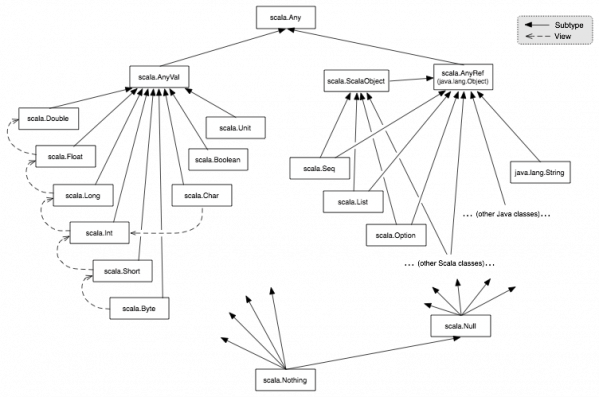
\includegraphics[width=10cm]{scala_type_hierarchy}
\caption{scala type hierarchy}
\end{figure}


\begin{itemize}
\item { \bf Any} is the base type of all types.
\item {\bf AnyVal} inherits from Any. Numeric types (boolean, Int) inherit from AnyVal
\item {\bf Any} defines methods '==','!=', toString
\end{itemize}

Nothing is at the bottom of scala's type hierarchy. it is a subtype of every other type.
Nothing can signal abnormal termination.
Empty lists/containers can have elememt type Nothing

Null is a subtype of all reference types, and the type of the null value
(null is the value, Null is the type)

% term rewriting?

% Class hierarchies - more than one class goes into the definintion of a derived class

\chapter{placeholder}
\section{ for comprehension}
backward arrows \lstinline|<-| call flatmap
final \lstinline|yield| calls map

\section{list functionality}
sublists and element access. The list \textbf{xs} has the following methods available
\begin{itemize}
  \item \textbf{xs.head} - first element in list
  \item \textbf{xs.tail} - remainder of list, with first element removed
  \item \textbf{xs.last} - last element of list
  \item \textbf{xs.init} - list containing all elements except first
  \item \textbf{xs.length} - number of elements in list
  \item \textbf{xs.take(n)} - sublist containing the first n elements of xs
  \item \textbf{xs.drop(n)} - sublist containing all remaining elements of xs, after the first n have been removed
  \item \textbf{xs(n)} - the nth element of list xs. The item access function is implemented through the apply function(xs.apply(n)), which can be invoked through just xs(n). 
  \item \textbf{xs.splitAt(n)} - splits the list at position $n$, returns two lists in a tuple
\end{itemize}
other list operations
\begin{itemize}
  \item \textbf{xs ++ ys} - concatenates xs and ys. This can also be done with the cons-like operator xs:::ys.
  \item \textbf{xs.reverse} - reverse the list
  \item \textbf{xs.updated.(n,x)} - replace the nth element with x
  \item \textbf{xs.indexOf(x)} - get the index of the first occurence of x (or -1 if x does not occur in xs)
  \item \textbf{xs.contains} - true if xs contains x, false otherwise
\end{itemize}

\section{Pairs and Tuples}
Some examples in  mergesort.sc \verb|week6/misc_worksheets/mergesort.sc|.

Functions can return multiple objects wrapped in a tuple, for example \href{https://www.scala-lang.org/api/2.12.3/scala/collection/immutable/List.html#splitAt(n:Int):(List[A],List[A])}{splitAt}:  \listInline| def splitAt(n:Int):(List[A],List[A])|. This returns a pair of lists, the first list contains the first $n$ elements of the original, the second contains the remaining elements. Pairs in scala can be written \lstinline|(x,y)|.

Pairs can be generalised to Tuples, which are collections of more than two elements.

A tuple is an instance of a parameterised scala type $\mathrm{scala.Tuple}N[T_1,...,T_N]$
The expression $(e_1,...e_N)$ is equivalent to $\mathrm{scala.Tuple}N(e_1,...e_N)$. Tuples can also be used in pattern matching.

TupleN classes follow the definition below
\begin{lstlisting}
case class Tuple2[T1,T2](_1: +T1,_2: +T2) {
  override def toString = "(" + _1 +", " + _2 + ")"
}
\end{lstlisting}
fields can be accessed by the names \lstinline|_1, _2| etc. As tuples are case classes, they can be used for pattern matching (see above worksheet).

\section{Implicit Parameters}

Would like to extend our mergesort to work on arbitrary parameter types. If we just specify a type parameter $[T]$ in the constructor (and don't do anything else), we'll get an error as the $<$ operator is not defined for all types. A solution is to take a function as an argument, and use that to make the $ x < y$ comparison.

There is, however, a class in the scala standard library that handles ordering - \lstinline|scala.math.ordering[T]| provides ways for ordering objects of type T

Instead of parameterising our function with a custom function for parameterisation, we could use Ordering for comparison instead:
\begin{lstlisting}
def msort_ord[T](xs:List[T])(ord: Ordering[T]): List[T] = {
...
case (x::xs,y::ys) => if (ord.lt(x,y)) x::merge(xs,y::ys) ...
...
merge(msort_ord(left)(ord),msort_ord(right)(ord)) }
}
msort_ord(myList2)(Ordering.String))
\end{lstlisting}

even better is to declare $ord$ as an $implicit$ parameter
\lstinline|def msort_ord[T](xs:List[T])(implicit ord: Ordering[T]): List[T] = ...|
Then ord no longer needs to be specified with the msort function is invoked. The compilier will figure out what should be used.
The compiler will search for an implicit definition that
\begin{itemize}
  \item is marked \lstinline|implicit|
  \item has a type compatible with \lstinline|T|
  \item is visible at the point of the function call, or is defined in a companion object associated with T.
\end{itemize}
If there is a single (most specific) definition, it will be taken as the argument. Otherwise an error will be thrown

\section{Higher order List functions}
\begin{itemize}
  \item \textbf{xs.map} - takes a function, returns a list formed by applying the function to each element of the list
  \item \textbf{xs.filter} - takes a function, returns a subset of the list containing all elements for which the function evaluates to true
  \item \textbf{xs.filterNot} - takes a function, returns a subset of the list containing all elements for which the function evaluates to false
  \item \textbf{xs.partition} - takes a function evaluating to bool, returns two lists, one containing elements that evaluate to true, the other elements that evaluate to false
  function evaluates to false
  \item \textbf{xs.takeWhile} - takes a function evaluating to bool, returns all elements up to (excluding) the first that evaluates to false
  \item \textbf{xs.dropWhile} - takes a function evaluating to bool, returns all elements after (including) the first that evaluates to false
  \item \textbf{xs.span} - takes a function evaluating to bool, returns two lists. The first list is equivalent to takeWhile, the second to dropWhile
\end{itemize}

  


















% syntax notation
% extended Backus-Naur form (EBNF)





